\documentclass{article}
\usepackage[UTF8]{ctex}
\usepackage{graphicx}
\usepackage{amsmath,amssymb,amsthm}
\usepackage[mathscr]{eucal}
\usepackage{rotate,graphics,epsfig}
\usepackage{mathrsfs}
\usepackage{geometry}
 \geometry{left=3.0cm,right=3.0cm,top=2.5cm,bottom=2.5cm}
\usepackage{natbib}
 \bibpunct[, ]{(}{)}{,}{a}{}{,}%
 \def\bibfont{\small}%
 \def\bibsep{\smallskipamount}%
 \def\bibhang{24pt}%
 \def\newblock{\ }%
 \def\BIBand{and}%
 
\newcommand{\nb}{\nonumber}
%opening
\title{基于隐马尔可夫模型的心梗阶段分析以及急性心梗事件预测}
\date{}
\author{
吴芷婧\quad \\
}

\begin{document}

\maketitle

\begin{abstract}
针对心梗后心脑血管不良事件的预测预警及优化治疗关键问题,构建预测预警的隐马尔可夫模型,给出相关指标体系与参数临界估计。基于易于观测的并发症信息,识别心梗病人病程不同发展阶段,并建立急性心梗事件的预警模型。
\end{abstract}
\section{研究背景}
心血管疾病死亡是中国城乡居民总死亡的首要原因,而其患病人数仍有快速增长之态势,其治疗费用也在逐年上升。根据《中国心血管健康与疾病报告2019》,每年约有350万人死于心血管疾病,其中心肌梗死患病人数高达250万。\par
《中国心血管病报告2018》概要[2]指出,今后十年间心血管病患病人数仍将快速增长。心血管疾病的治疗费用也呈逐年上升之趋势。统计分析结果显示[5],心肌梗死患者的人均费用从2014年的30581.51元增长至2018年的37757.72元,年均复合增长率5.41\%,住院费用平均水平为34814.62元。\par
心肌梗死患者病情重、变化快,对护理人员的观察能力和处置能力有着更高的要求。在心肌梗死患者护理工作量日益增加、专业化发展不断推进而年轻护士不断增加的新形势下,由于现行工作模式缺乏客观、定量、智能预警系统,存在心梗后心血管意外事件预见性差、临床处置不得当、护理不良事件不断增加等问题。心梗后心血管不良事件的增加,又进一步增加了患者的治疗费用。有研究指出,构成心肌梗死患者高额费用的主要原因在于患者因病情恶化需要抢救一次或者多次而产生的手术费用和材料费用,抢救存活后稳定病情所需的药品费以及观察病情变化而产生的检查费。因此,本项目拟建立心脑血管不良事件的早期预警模型,对于危重病人的病情变化,提早从微妙的状态波动中发现识别,早确认早干预早治疗。
\par
国内外对于心血管疾病的研究虽然已经建立了规模庞大的前瞻性队列,但这些队列研究结论往往基于流行病学的统计分析,从人口学信息、既往疾病史、家族疾病史以及一些健康危险因素的角度,宏观评估人类心血管疾病的患病风险,并进行长时间的跟踪调查,对心血管疾病的远期生存率回访研究,建立长期心血管疾病慢性病变的综合认知。而临床上心血管疾病特别是心梗后病人病情的快速演变具有时效性强,不确定性因素等特点,流行病学及回归分析不能很好的满足实际应用的需要并且包含人口学信息、既往疾病史、家族疾病史等的简单样本数据不足以支撑对于病人病情演变的模拟。精细而深入的研究复杂性疾病的科研和决策需要更大的样本量和更为准确全面的测量,本项目拟利用大数据进行心血管专病研究的分析和挖掘,从时序进程、概念范畴两个维度对心血管疾病风险预测进行进一步探究使,大数据真正转化为科研成果,提供方便临床应用的方案,达到预警时间提前,不良事件率下降的目的,从而真正提高科研创新能力和医疗服务能力,提高病人病后的生活幸福指数,并最终促进临床医学研究的发展。
\par
数学建模及人工智能具有为心梗后心脑血管事件提供早期预警的潜能。为心梗后心脑血管事件提供早期预警,需要对病情发展态势进行刻画,了解病情发展过程,预测未来发展规律。数学建模的特点在于在专业医学知识的加持下,可以将心梗后心脑血管事件进行抽象刻画,明确病情发展规律,提供准确的病情预测,从而帮助患者早发现,早治疗,提高生活幸福指数。人工智能的发展为数学模型落地到实际应用中提供了强有力的支持。人工智能可以挖掘未被发现的患者病情要素间的医学联系,帮助医生识别肉眼难以发现的病情指征,为数学模型提供了重要的输入指标;人工智能算法在大数据上性能表现也为将数学模型落地到实际应用提供了可能。
\par
由于心梗后心脑血管事件的复杂性及特异性,将数学建模及人工智能应用到心梗后心脑血管事件的早期预警及诊疗具有很高的难度。由于心梗后心脑血管事件病例机制的复杂性,相关的医疗数据具有高维度和高缺失率,为数学建模参数估计带来了很大的困难。为保证模型的移植性,即模型在不同数据上都可以表现出很好的结果,这就需要在数学建模及创建人工智能算法中认真处理数据高维度和高缺失率的难点。其次,为病人提供优化的诊疗方案,需要我们建立动态决策模型并提供优化策略,即在不同的病情状态下,为病人选择最优的治疗方案,这在数学建模上本身就具有一定的难度。
\par
因此我们的研究致力于解决在心梗后心脑血管事件上数学建模及创建人工智能算法上的困难,为病人提供早期预警模型,并提供优化的诊疗方案。从群体防治角度而言,该模型致力于筛选心血管风险高危人群和患者,以便尽早确立以降低心血管绝对风险为目标的预防治疗策略,实现“早发现,早治疗”的心血管疾病管理目标。从临床医护的患者管理角度而言,该心梗后心脑血管事件预测模型致力于成为临床医师制定个体化治疗方案的重要依据,帮助医务人员对高危个体进行健康教育和健康管理。从患者及高危人群本身角度而言,该模型致力于加强个体自我风险评估的意识,为早期预防心梗后心血管时间的发生、提高我国居民健康水平做出贡献。

\section{文献回顾}
\subsection{心梗后心脑血管事件早期预警及诊疗的医学研究进展}
心血管疾病风险评估的概念与设想最早由美国提出,考虑到不同人种的差异性,适用于不同人种的风险预测模型接踵而出。美国依据Framingham队列研究开发了冠心病发病预测模型,此后又陆续开发了各种心血管疾病的风险评估工具,以分析心血管疾病及其危险因素。其中以1998年发布的冠心病Framingham危险评分(FRS)影响最为广泛,采用的分析方法主要包括直接评分法和多元回归方法,纳入的危险因素主要包括年龄、血压、低密度脂蛋白胆固醇、高密度脂蛋白胆固醇、家族史和吸烟等。由于FRS模型会高估欧洲心血管疾病发病风险,因此,为了构建适用于欧洲心血管疾病发病风险的评估模型,欧洲心血管协会集成了来自12个欧洲国家的具有代表性的研究队列资料建立起一种新的心血管疾病风险评估模型——Score模型。Score模型把心血管疾病死亡作为终点事件,旨在评估10年致死性心血管病风险。该模型以一种更接近于临床实践的形式,提供了对致命性心血管风险的直接估计方法。另一方面,为了建立适用于英国人的心血管疾病风险评估模型,英国以Cox风险回归为主要分析方法建立了英国Qrisk心血管风险评估系统 (QRFSEARCH Cardiovascular Risk Algorithm)。Qrisk将冠心病、心肌梗死、卒中、心绞痛以及短暂性脑缺血发作作为终点事件,纳入的危险因素除FRS模型中包含的传统的危险因素如年龄、性别、血压、吸烟史、体重指数、高密度脂蛋白胆固醇、总胆固醇之外,还纳入了地区及社会剥夺等新的危险因素[6]。
近年来,国内也积极开展了一些关于心血管疾病风险评估方面的研究。如中国人群动脉粥样硬化性心血管疾病(ASCVD)发病风险预测研究(China-PAR)[7],整合了我国4项最新前瞻性队列随访数据,总样本量达12.7万人,最长随访时间超过23年。其采用Cox风险比例回归模型,按照性别分别创建了心脑血管疾病发病风险预测模型。经过验证,China-PAR对10年和15年发病风险均有良好的预测能力。
\subsection{数学建模及人工智能在医学应用上的发展及不足}
由于大数据的驱动,近年来,数学建模及人工智能在医疗诊断及治疗优化的研究呈现出多角度、多领域的创新研发局面。这些应用包括原发性肺结节诊断、新型冠状病毒肺炎患者胸片及CT的识别、糖尿病视网膜病变的自动检测、皮肤癌的分类及乳腺癌患者中转移性淋巴结病的检测等。但是关于心梗后心脑血管事件的早期预警和诊疗还缺乏相应的研究。因此,本课题旨在通过数学模型建立心梗后心脑血管事件的早期诊断诊断,提供可推广的早期预警方案,并进一步提供针对性的优化诊疗方案。

\section{模型建立}
\subsection{模型概述}
为建立急性心梗事件早期预警模型,考虑到部分病人底层的心梗病程阶段的不可直接观测性,我们采用隐马尔可夫模型(Hidden Markov Model, HMM)。隐马尔可夫模型(HMM)是一种马尔可夫链,其状态无法直接观测,需要通过一些可观测现象的向量序列进行分析。在我们研究中,由于病人的心梗类型和病程发展状况需要很高的成本才能精确判断,医院往往只能通过可直接观测到的包括心梗后的心血管事件的临床数据、X片和CT影像等数据进行推断。考虑到现实情况,一方面,心肌梗塞的各个阶段和类型判断需要耗费一定的成本;另一方面,不同的可观测的心脑血管事件在心梗患者的不同病程阶段都有可能出现。因此,我们采用隐马尔可夫模型(Hidden Markov Model,HMM)刻画病人的病程发展阶段,并对病人可能出现的心脑血管事件进行预测,最终打造多模态大数据背景下的识别-预警一体化模型框架。
\par 
具体到模型建立,我们首先将病人表象的心血管事件与其底层的心梗病程发展阶段关联起来;然后基于我们的多模态数据支持,利用人工智能技术学习患者各种医疗数据与心梗类型的相关性,对相关指标进行参数临界值估计,由于我们的数据具备多模态、多维度、海量性等特点,可以采用神经网络这一项技术手段进行处理和分析;最后基于第一步心梗类型与心梗后心脑血管事件的相关性结果,以及第二步患者各种医疗数据与心梗类型的相关性结果,我们可以基于病人的医疗数据对病人发生不同心梗后心脑血管事件进行预测,建立心梗后心脑血管事件早期预警模型,通过输入病人病情相关参数,即可预测病人心梗后不同心脑血管时间发生的概率。
\par

\subsection{模型定义}
\subsubsection{VD-HMM模型}
我们在传统HMM模型的基础上,加入不同心梗阶段的持续时长,得到VD-HMM模型(Variable-Duration Hidden Markov Model),以便更加准确地描述心梗阶段及其转移,从而提高模型的拟合和预测效果。我们关于急性心梗预测的VD-HMM 模型共包含五部分。(1)通过文本分析得到的疾病的观测结果,即并发症组合;(2)疾病的隐藏状态,即心梗阶段;(3)心梗阶段与观测结果的对应,即输出概率矩阵;(4)心梗阶段的持续时间;(5)利用心梗阶段预测急性心梗的发病概率。\par

\begin{center}
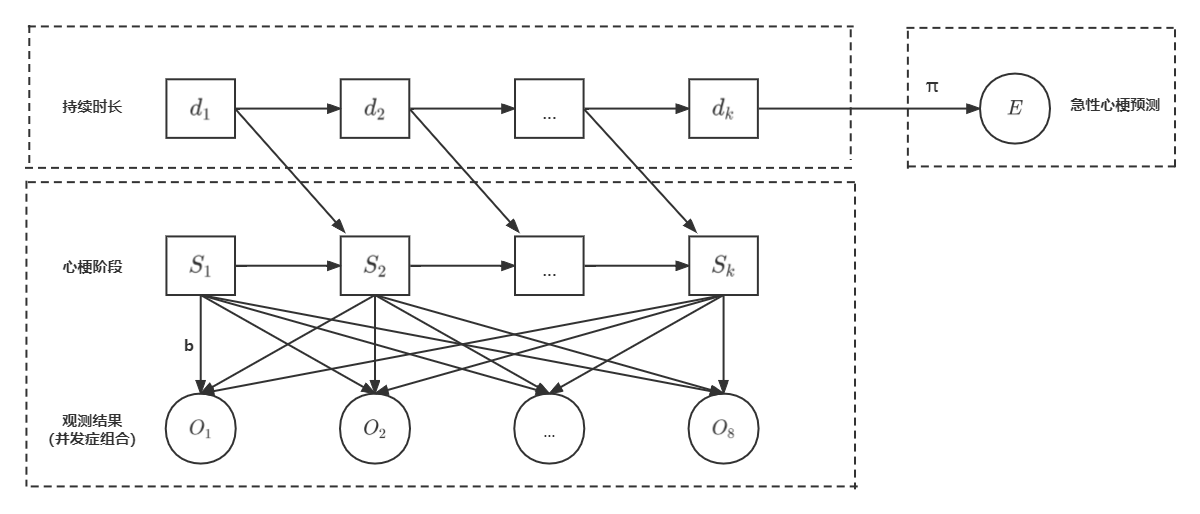
\includegraphics[width=0.8\textwidth]{VDHMM模型.png}\\
\text{图1:VD-HMM模型}
\end{center}

如图1所示,$O$ 代表并发症组合,我们根据病人诊疗记录中的“病情描述”与“出院诊断”进行文本分析,利用回归模型筛选出具有决定作用的并发症,得到并发症组合。$O_{ij}$表示病人$i$第$j$次问诊的所表现的并发症组合。 $S$代表不同的心梗阶段,由于心梗阶段不可直接观测,故属于隐藏状态,又由于目前对心梗阶段尚未有明确的划分标准,其阶段数量$k$也尚待确定。$b$代表输出概率,即$b_s(o) =P(O_{ij}=o|S_{ij}=s) $刻画处于不同心梗阶段$s$时病人出现某一并发症组合$o$的可能性。$d_m$代表某病人在每一心梗阶段病情持续的时间。心梗阶段与持续时长共同决定心梗状态的转移函数。$E$通过对模型的输出结果的分析,预测得到的该病人急性心梗的发病可能性。

\subsubsection{观测空间定义:并发症组合}

在隐马尔可夫模型当中,由于入院病人的并发症是易于识别与观测的,我们采用不同的并发症组合作为观测空间中的元素。在定义关键并发症的过程中,我们从1266条诊断记录的“现病史”、“病情描述”、“初步诊断”三列文字描述中,根据词频统计的方法,选择出出现频率最高的“胸闷”、“狭窄”、“胸痛”、“头晕”、“中段”、“呕吐”、“不适”、“恶心”八个并发症相关词语,并对“胸闷”、“狭窄”、“胸痛”、“头晕”、“中段”、“呕吐”、“不适”、“恶心”进行正则化匹配。将该8个分词描述作为自变量输入、诊断结果作为因变量输出,分为非急性心梗(陈旧性心梗)-0与急性心梗(表格1中其余三项),建立Logistic回归模型,选择与急性心梗事件偏相关性较高的并发症。\par

\begin{center}
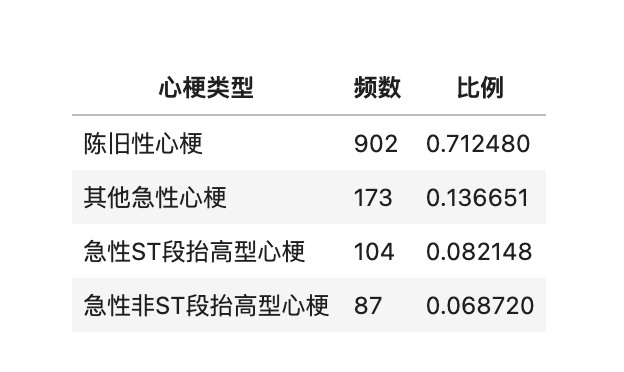
\includegraphics[width=0.6\textwidth]{心梗类型.png}\\
\text{表1:急性与非急性心梗分类}
\end{center}
Logistic回归结果如下表所示:
\begin{center}
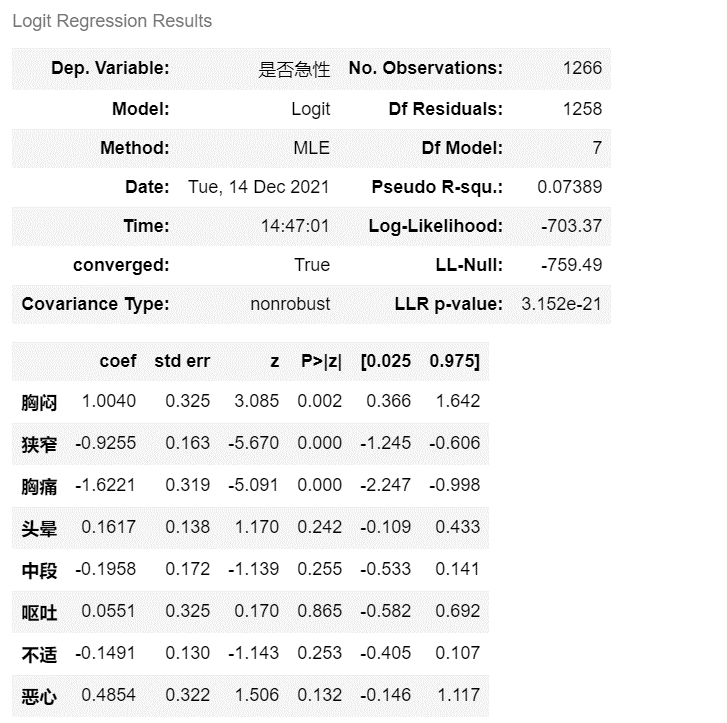
\includegraphics[width=0.8\textwidth]{分词回归.png}\\
\text{图2:Logistic回归结果}
\end{center}
根据Logistic回归结果,我们选择“胸闷”“狭窄”“胸痛”作为关键自变量,选择并发症组合作为观测空间中的元素,编码结果如表格2所示。
\begin{center}
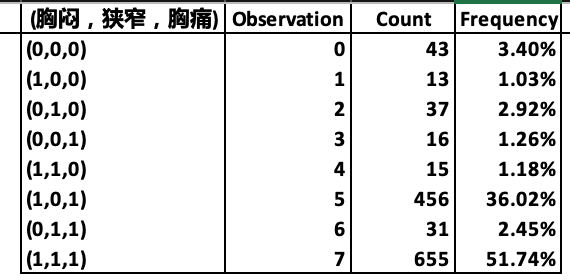
\includegraphics[width=0.6\textwidth]{观测空间.png}\\
\text{表2:并发症组合编码与观测空间定义}
\end{center}

\subsubsection{输出概率矩阵}
我们采用并发症组合定义离散观测空间,因此采用刻画离散型随机变量的多项式分布对输出概率矩阵进行参数化建模。
$$
b_s(o_1,\cdots, o_M)=\left(\begin{array}{c}
n_s \\
o_{1} \cdots o_{M}
\end{array}\right) p_{1,s}^{o_{1}} \cdots p_{M,s}^{o_{M}},\ for\ s\ \in \{1,\cdots, N\}.
$$

其中输出概率矩阵中的元素$b_s(o_1,\cdots, o_M) = P(O_1=o_1,\cdots,O_M=o_M|S=s)$表示了给定入院病人所处状态(病程发展阶段)时,出现各个观测(并发症组合)的联合概率,而对于这一概率,我们借助多项式分布的联合概率质量函数的结构对其进行参数化,对应的待估参数为$\{(p_{1,s},\cdots,p_{M,s})|s=1,\cdots,N\}$。


\subsubsection{转移概率矩阵}
转移概率矩阵描述了病人从一个病情阶段转移到新的阶段(恶化或减轻)的概率。在传统的HMM模型中,转移到新状态的概率仅取决于当前的状态,即考虑离散马尔可夫过程的一步转移概率矩阵;而本模型另考虑了两次转移的间隔时间、在当前状态存续时间、入院病人的其他特征信息对转移的影响,即采用Logistic回归形式对转移概率函数进行参数化建模,考虑更为复杂的连续时间马尔可夫过程的转移规律。\par

我们将转移概率分为两部分,一部分是在原状态的滞留,
即${S_{i,j+1} = s| S_{i,j} = s}$;
另一种是向新状态的转移,
即${S_{i,j+1} = s'| S_{i,j} =s}$。
此处我们假设在原状态滞留的概率为$p$,则向其他状态转移的概率为$1-p$,并对在原状态滞留的概率建模如下。
\par
\begin{equation}
	\begin{aligned}
% 		& 
		p_{ss}(d_j,\Delta_{j,j+1},\sigma_{ij})
% 		\\	& 
		= logit^{-1}[\lambda_0^s + \lambda_1 log(1+d_j(s)) - log(\Delta_{j,j+1}) + \lambda_3\sigma_{ij}) ]
	\end{aligned}
\end{equation}\par
对于原状态停留的概率,其取决于以下多个因素。首先,在不同的心梗阶段中,病人滞留的时间会有所不同,例如病人更难以从更加严重的心梗状态中转移(恢复),而病情轻微的病人可能需要更长时间才会恶化到下一阶段。我们用$\lambda_0^s\ (s=1,2,...)$表示不同心梗阶段对停留概率的影响。变量$\Delta_{j,j+1}$表示病人两次入院检查所间隔的时间,体现了病人问诊的频率,我们也可以由此推算出病人在不同心梗状态中滞留的时间。因此$\lambda_2$表示病人问诊频率对转移概率的影响。变量$d_j(s)$表示病人第$j$次问诊所处的状态已存续的时间,故$\lambda_1$体现了前文所述的持续时长对状态转移的影响。另外,由于病人的病情发展情况也收到个体差异的影响,我们用$\sigma_{ij}$描述个体差异(第i个病人第j次入院的身体情况),用$\lambda_3$表示个体差异的影响。综上,我们使用Logistic模型表示逗留概率$p$。
\par

对于状态$s$向新状态$s'$的转移,其概率可以表示为$(1-p)\Gamma_{ss'}$
其中$\Gamma_{ss'}\in [0,1]$且$\sum_{s'\neq s}^{N}\Gamma_{ss'}=1$。综合两种转移情况,转移概率可以表示为:
\begin{equation}
	 P(S_{i,j+1} = s'| S_{i,j} = s,d_j)
	 =
	\begin{cases}
     	& p_{ss}(d_j,\Delta_{j,j+1},\sigma_{ij}) \qquad s'=s\\	
		& (1-p_{ss}(d_j,\Delta_{j,j+1},\sigma_{ij}))\Gamma_{ss'} \qquad s'\neq s
	\end{cases}
\end{equation}\par

在对转移概率函数进行参数化之后,对应的待估参数为$\{(\lambda_0^s,\lambda_1,\lambda_3,\Gamma_{ss'})|\Gamma_{ss'}\in [0,1],\sum_{s'\neq s}^{N}\Gamma_{ss'}=1 ,s,s'=1,\cdots,N\}$。

\section{模型参数估计}
由于目前我们仅能够获取病人的入院时间,无法精确判断病人病程发展发生变化的时间,即无法精确获取连续时间马尔可夫链的嵌入链信息;由于病人未必定期前往医院,我们也无法采用“h-离散骨架”来分析连续时间马尔可夫链。因此,在本课题研究中,我们暂时考虑选择离散时间马尔可夫链作为我们的模型基础,并且将转移函数简化为一步状态转移矩阵,将急性心梗事件预测问题自变量中的持续时间项换为表示病人所处病程阶段(状态)的示性函数。


\subsection{离散时间隐马尔可夫模型参数}
$$\lambda=(N,M,\pi,A,B)$$

$N$:状态空间的元素个数。

$M$: 观测空间的元素个数。

$\pi$: 状态的初始分布。

$A$: 离散HMM转移概率矩阵。

$B$: 离散HMM输出概率矩阵。

\subsection{回归参数}

$$ logit(P(Y_{ij}=1|s_{ij},Z_{ij}))=w_0+\sum\limits_{s=1}^N w_s \mathcal{I}(s_{ij}=s)+w^T_Z\cdot Z_{ij}$$

其中$\{(w_0,w_Z,w_s)|s=1,\cdots,N\}$为待估的回归参数。$\mathcal{I}$为示性函数。$Z_{ij}$为第i个病人在第j次看病中的其它协变量,如年龄、性别等。

\subsection{极大似然估计方法}

\begin{eqnarray}
    L(w,\lambda)&=&\sum\limits_{i=1}^{I} \log(P(O_{i1},\cdots,O_{iJ_{i}},Y_{i1},\cdots,Y_{iJ_{i}}~|~w,\lambda))\nb\\
    &=&\sum\limits_{i=1}^{I} \log(P(\bar{O_{i}},\bar{Y_{i}}~|~w,\lambda))\nb\\
    &=&\sum\limits_{i=1}^{I} \log(P(\bar{Y_{i}}~|~\bar{O_{i}},w,\lambda))\\
    &+& \sum\limits_{i=1}^{I}\log(P(\bar{O_{i}}~|~\lambda))
\end{eqnarray}

(3)式可以重新写为
\begin{eqnarray}
&&\sum\limits_{i=1}^{I} \log(P(\bar{Y_{i}}~|~\bar{O_{i}},w,\lambda))\nb\\
&=&\sum\limits_{i=1}^{I}\log(\sum\limits_{\bar{s}_i}P(\bar{Y_{i}}~|~\bar{s_i},\bar{O_{i}},w,\lambda)P(\bar{s_i}~|~\bar{O_{i}},w,\lambda))\nb\\
&=&\sum\limits_{i=1}^{I}\log(\sum\limits_{\bar{s}_i}P(\bar{Y_{i}}~|~\bar{s_i},w)P(\bar{s_i}~|~\bar{O_{i}},\lambda))\nb\\
&\geq&\sum\limits_{i=1}^{I}\log(P(\bar{Y_{i}}~|~\bar{s_i}^*,w))+\sum\limits_{i=1}^{I}\log P(\bar{s_i}^*~|~\bar{O_{i}},\lambda)
\end{eqnarray}

其中(4)式中,可利用$Baum-Welch$算法,选取$\hat{\lambda}=\arg\max(\sum\limits_{i=1}^{I}\log(P(\bar{O_{i}}~|~\lambda)))$,作为隐马尔可夫模型参数$\lambda$的估计。

其中(5)式中,可利用$Vilerbi$算法,选取$\bar s_i^*=\arg\max_{\bar s_i} P(\bar{s}_i~|~\bar{O}_i,\lambda)$,作为隐马尔可夫模型的隐藏状态的估计;可利用极大似然估计的方法,选取  $\hat{w}=\arg\max_{w} \sum\limits_{i=1}^{I} \log P(\bar{Y}_i~|~\bar{s}_i^*,w)$ ,作为心梗急性事件的回归预测模型的参数估计。


\section{模型参数估计结果}
\subsection{基于并发症的急性心梗事件预测}
本课题选择没有采用隐马尔可夫模型,仅考虑关键并发症(胸闷、血管狭窄、胸痛)的Logistic回归作为基准模型,此模型结果如表3。
\begin{center}
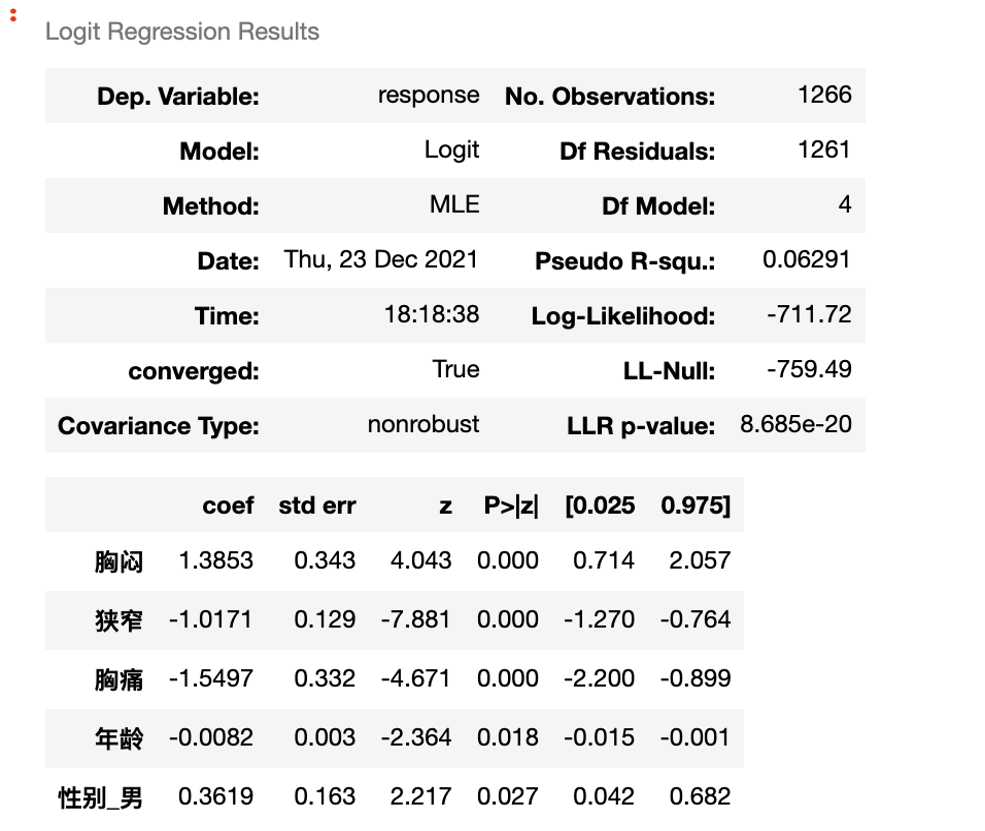
\includegraphics[width=0.8\textwidth]{LR_benchmark.png}\\
\text{表3:基于并发症的急性心梗事件预测,基准模型}\\
\end{center}
分析模型各项系数,我们发现“胸闷”一项系数为正(1.39),且对应p值说明系数不显著为零,说明给定其他变量不变,出现“胸闷”的患者出现急性心梗事件的概率优势为未出现“胸闷”患者的4倍。
在拟合优度方面,将本模型的预测值与真实值比较,预测精度为71.88\% ;模型的伪$R^2$为0.063。

\subsection{选择状态空间元素个数为4}
根据第四版“心肌梗死全球定义”的标准,心肌梗死可分为以下5型:
\begin{itemize}
    \item 1型:由冠状动脉粥样硬化斑块急性破裂或侵蚀,血小板激活,继发冠状动脉血栓性阻塞,引起心肌缺血、损伤或坏死,同时须具备心肌损伤和至少一项心肌缺血的临床证据;
    \item 2型:为心肌供氧和需氧之间失平衡所致心肌梗死,与冠状动脉粥样硬化斑块急性破裂或侵蚀、血栓形成无关;
    \item 3型:指心脏性死亡伴心肌缺血症状和新发生的缺血性心电图改变或心室颤动,但死亡发生于心脏生物标志物的血样本采集之前或发生于心脏生物标志物明确升高之前,尸检证实为心肌梗死;
    \item 4型:包括经皮冠状动脉介入治疗(percutaneous coronary intervention,PCI)相关心肌梗死(4a型)、冠状动脉内支架或支撑物血栓形成相关心肌梗死(4b型)及再狭窄相关心肌梗死(4c型);
    \item 5型:为冠状动脉旁路移植术(coronary artery bypass grafting,CABG)相关心肌梗死。
\end{itemize}

由于我们的数据中并没有出现死亡的病例,不考虑心梗5型划分中的第3型心梗,我们认为将心梗病程发展划分为4个阶段较为合理。

采用4.3中极大似然方法,我们获得离散时间隐马尔可夫过程的初始分布、转移概率矩阵、输出概率矩阵如下表所示。
\begin{center}
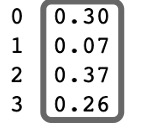
\includegraphics[width=0.15\textwidth]{初始分布4.jpeg}\\
\text{表4:离散时间隐马尔可夫过程初始分布,N=4}\\
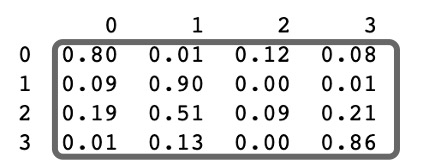
\includegraphics[width=0.4\textwidth]{转移概率矩阵4.jpeg}\\
\text{表5:离散时间隐马尔可夫过程转移概率矩阵,N=4}\\
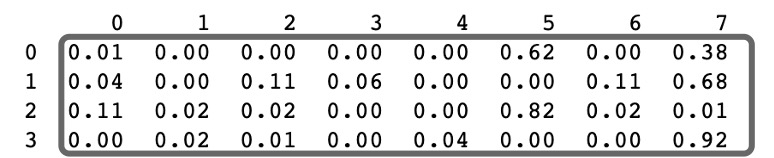
\includegraphics[width=0.8\textwidth]{输出概率矩阵4.jpeg}\\
\text{表6:离散时间隐马尔可夫过程输出概率矩阵,N=4}
\end{center}

采用$Viterbi$算法得到的每个病人每次最可能处于的病程发展状态,并在此基础上建立Logistic回归模型,模型结果如表7。

\begin{center}
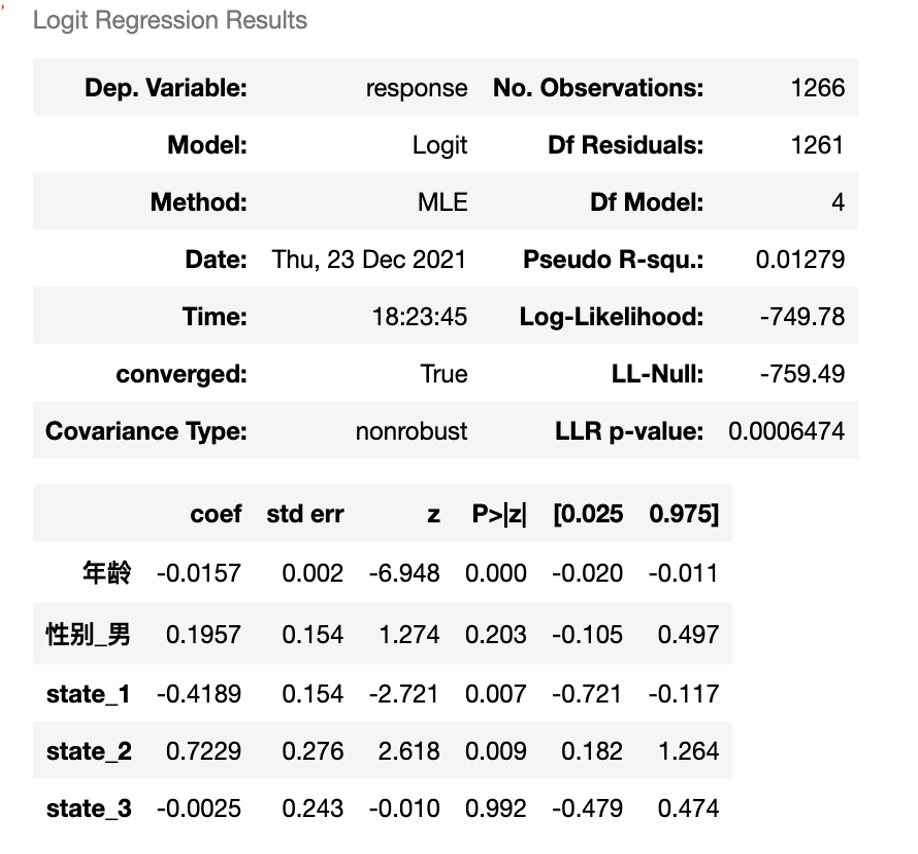
\includegraphics[width=0.8\textwidth]{LR_4.png}\\
\text{表7:基于隐状态的急性心梗事件预测,N=4}\\
\end{center}

分析回归结果中各项系数,由于“状态3”对应的p值超过0.05,在0.05的显著性水平下,无法拒绝此项对应的系数为零的假设,因此我们重新选择状态空间元素个数,重新建模。
在拟合优度方面,将本模型的预测值与真实值比较,预测精度为71.64\% ;模型的伪$R^2$为0.013。相较于基准模型,预测精度有轻微下降,伪$R^2$明显下降。


\subsection{选择状态空间元素个数为3}

采用4.3中极大似然方法,我们获得离散时间隐马尔可夫过程的初始分布、转移概率矩阵、输出概率矩阵如下表所示。
\begin{center}
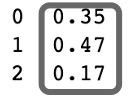
\includegraphics[width=0.15\textwidth]{初始分布3.jpeg}\\
\text{表8:离散时间隐马尔可夫过程初始分布,N=3}\\
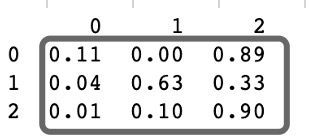
\includegraphics[width=0.4\textwidth]{转移概率矩阵3.jpeg}\\
\text{表9:离散时间隐马尔可夫过程转移概率矩阵,N=3}\\
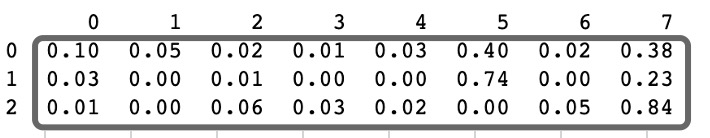
\includegraphics[width=0.8\textwidth]{输出概率矩阵3.jpeg}\\
\text{表10:离散时间隐马尔可夫过程输出概率矩阵,N=3}
\end{center}

采用$Viterbi$算法得到的每个病人每次最可能处于的病程发展状态,并在此基础上建立Logistic回归模型,模型结果如表11。

\begin{center}
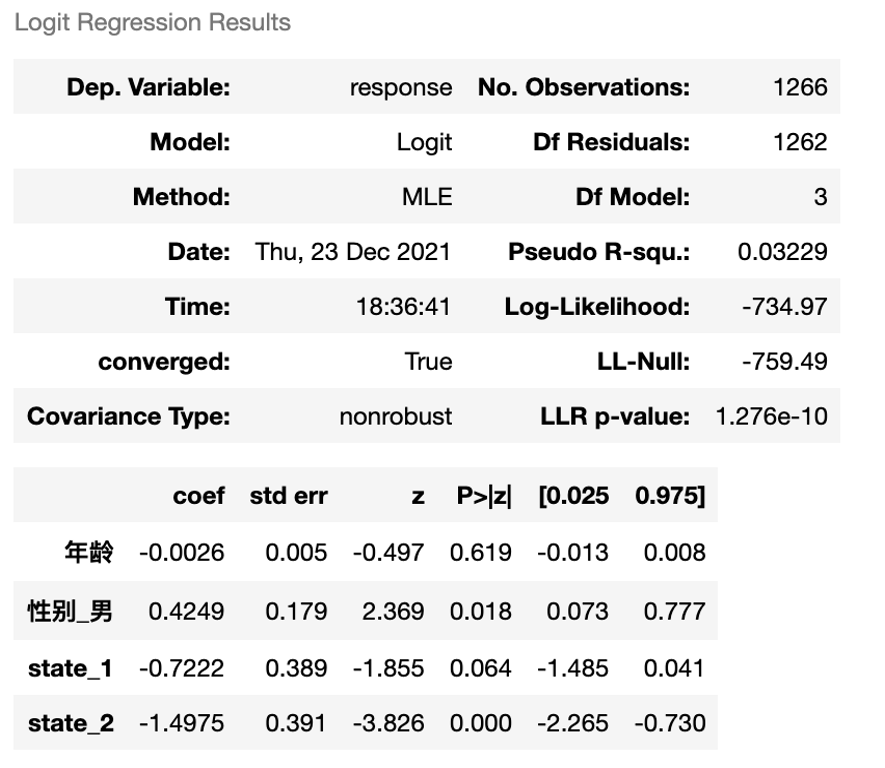
\includegraphics[width=0.8\textwidth]{LR_3.png}\\
\text{表11:基于隐状态的急性心梗事件预测,N=3}\\
\end{center}

分析回归结果中各项系数,我们发现“状态1”一项系数为负(-0.722),且对应p值说明系数不显著为零,说明给定其他变量不变,处于“状态1”的患者出现急性心梗事件的概率优势为处于“状态0”患者的0.49倍;我们发现“状态2”一项系数为负(-1.498),且对应p值说明系数不显著为零,说明给定其他变量不变,处于“状态2”的患者出现急性心梗事件的概率优势为处于“状态0”患者的0.22倍。

在拟合优度方面,将本模型的预测值与真实值比较,预测精度为71.56\%,较基准模型有所下降,这是由于估计隐马尔可夫模型参数造成了一定的误差 ;模型的伪$R^2$为0.032。相较于基准模型,也有所下降。说明此方法在提升模型的解释能力的同时,也牺牲了一定的预测精度。

根据回归分析结果,我们知道“状态0”为病人病程发展中的“较严重状态”,“状态1”为“中度状态”,“状态2”为“轻度状态”。根据表8初始分布,我们了解到,较多的第一次入院病人处于“较严重状态”与“中度状态”,较少的病人处于“轻度状态”。

根据表9转移概率矩阵,我们了解到,“轻度状态”的病人在经历入院诊断与治疗后(包括下次诊断前的院外生活中),有较大的概率(0.9)处于原状态,有一定的概率(0.1)转移至“中度状态”,有极低的概率会发展至“较严重状态”。“中等状态”的病人在经历入院诊断与治疗后(包括下次诊断前的院外生活中),有较大的概率(0.63)仍停留在原状态,有较大的概率(0.33)恢复至“轻度状态”,也有一定的概率发展至“较严重状态”。处于“较严重状态”的病人在经历入院诊断与治疗、以及下次诊断前的恢复期后,有较大的概率(0.89)恢复至“轻度状态”,也有一定的概率(0.11)仍处于原状态。

根据表10输出概率矩阵,我们了解到,“轻度状态”下的患者很可能(0.84)同时出现胸闷、血管狭窄、胸痛的症状;“中度状态”下的患者很可能(0.74)同时出现胸闷、血管狭窄的症状;“较严重状态”下的患者并发症情况较为复杂。


\section{未来研究方向}
本课题研究目前在离散时间马尔可夫过程的框架下分析心梗病人的心梗阶段发展与不良事件的预警,并且在急性心梗事件的预测中除了并发症信息,仅考虑了年龄、性别两个协变量。在未来的研究当中,我们计划从更新模型参数估计方法、考虑更多的协变量、考虑连续时间马尔可夫过程、考虑病人在每个心梗阶段的持续时间几个角度,进一步提高模型精度。

除了并发症信息,我们计划纳入更多的危险因素信息(协变量)。除了FRS模型中包含的传统的危险因素如年龄、性别、血压、吸烟史、体重指数、高密度脂蛋白胆固醇、总胆固醇之外,课题还计划考虑地区及社会剥夺等新的危险因素,以及图片、音频等多模态大数据。一方面,我们将在急性心梗事件的预测问题中考虑更多的协变量,提高分类模型的预测精度;另一方面,我们也希望在隐马尔可夫过程的转移函数中引入刻画病人身体状况的协变量,使得马氏过程的转移更贴近病人真实病程发展状况。

采用连续时间马氏过程分析心梗病人的心梗阶段发展。目前由于我们只有病人的入院诊断时间,无法明确刻画隐马尔可夫过程(心梗发展过程)的状态转移间隔时间与状态逗留时间,暂时选择离散时间马尔可夫过程建模。接下来我们需要考虑如何更为精确地判断病人的状态转移时间与状态逗留时间,或者用每两次入院诊断的间隔时间进行近似,采用VD-HMM的框架分析连续时间隐马尔可夫过程的转移概率函数,并在急性心梗时间的预测问题中新增考虑各个状态的逗留时间。

在模型参数的估计方面,我们计划找到使似然函数最大化的一组参数$(\lambda,w)$。目前我们仅找到一种方法,结合Viterbi算法、Baum-Welch算法,完成似然函数的某一下界的最大化,但未来我们希望从新设计算法,结合向前-向后算法与Baum-Welch算法,找到使似然函数本身最大化的一组参数。




\newpage


\begin{thebibliography}{99}
\bibitem CChristof Naumzik, Stefan Feuerriegel, Markus Weinmann. I Will Survive: Predicting Business Failures from Customer Ratings. Marketing Science, 2021.

\bibitem  
CKRISTIAN THYGESEN, JOSEPH S. ALPERT, ALLAN S. JAFFE, et al. Fourth Universal Definition of Myocardial Infarction (2018)[J].  Journal of the American College of Cardiology,2018,72(18):2231-2264.

\bibitem C胡盛寿,高润霖,刘力生,等.《中国心血管病报告2018》概要[J].中国循环杂志,2019,34(3):209-220.

\bibitem C中华医学会心血管病学分会,中华心血管病杂志编辑委员会.急性ST段抬高型心肌梗死诊断和治疗指南(2019)[J].中华心血管病杂志,2019,47(10):766 783.

\bibitem
C中华医学会心血管病学分会,中华心血管病杂志编辑委员会.非ST段抬高型急性冠状动脉综合征诊断和治疗指南(2016)[J].中华心血管病杂志,2017,45(5):359 376.

\bibitem C黄广成,张远妮,邓光璞,等.急性心肌梗死患者住院费用的影响因素研究[J].中国卫生统计,2021,38(1):124-127.

\bibitem C马兴录,杨文文,冯云霞. 心血管疾病风险评估研究综述[J]. 计算机应用,2018,38(z2):111-114.

\bibitem 
CYANG, XUELI, LI, JIANXIN, HU, DONGSHENG, et al. Predicting the 10-Year Risks of Atherosclerotic Cardiovascular Disease in Chinese Population The China-PAR Project (Prediction for ASCVD Risk in China)[J].  Circulation: An Official Journal of the American Heart Association,2016,134(19):1430-1440. 

\end{thebibliography}



\end{document}
